Nesta seção explicamos as duas integrações que fizemos com exercícios-programas dados em disciplinas de introdução a computação e que envolviam física.

\subsection{Configuração}


os enunciados estão


\subsection{Angry Bixos}

\begin{itemize}
  \item yE , vmax : 2 reais que definem a posição do estilingue e a velocidade máxima com que um bixo pode ser arremessado;
  \item yA , hA : 2 reais que definem a posição do alvo e sua altura;
  \item dist: real positivo que define a distância xA − xE entre o alvo e o estilingue.
  \item nBix: inteiro que define o número de bixos que podem ser lançados;
  \item nLin, nCol: 2 inteiros que definem as dimensões do gráfico a ser impresso (ambos devem ser múltiplos de 5);
  \item nUni: real utilizado como fator de escala das alturas (número de unidades de altura por linha);
  \item g: real negativo que define a aceleração da gravidade.
\end{itemize}

\begin{figure}[H]
    \centering
	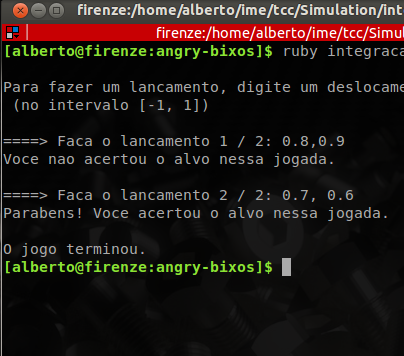
\includegraphics[scale=0.6]{images/angry-bixos-3.png}
	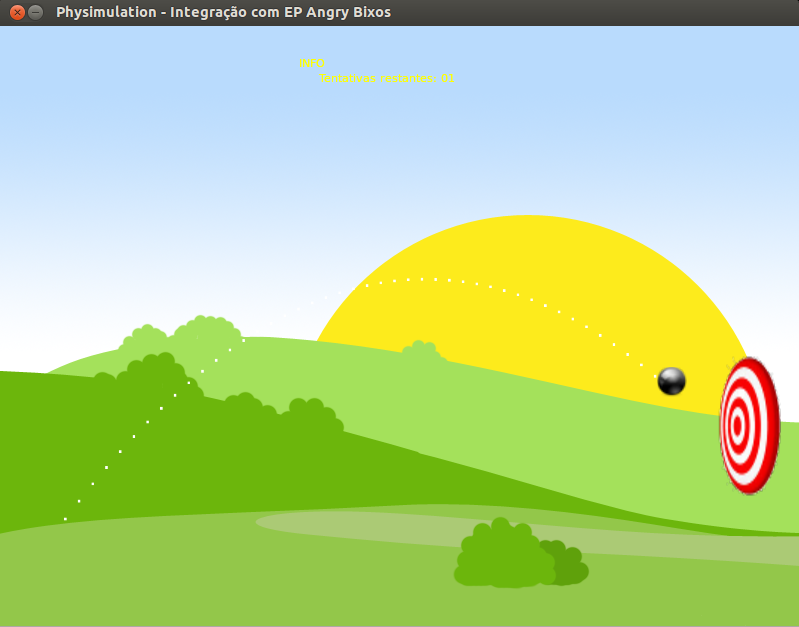
\includegraphics[scale=0.22]{images/angry-bixos-4.png}
	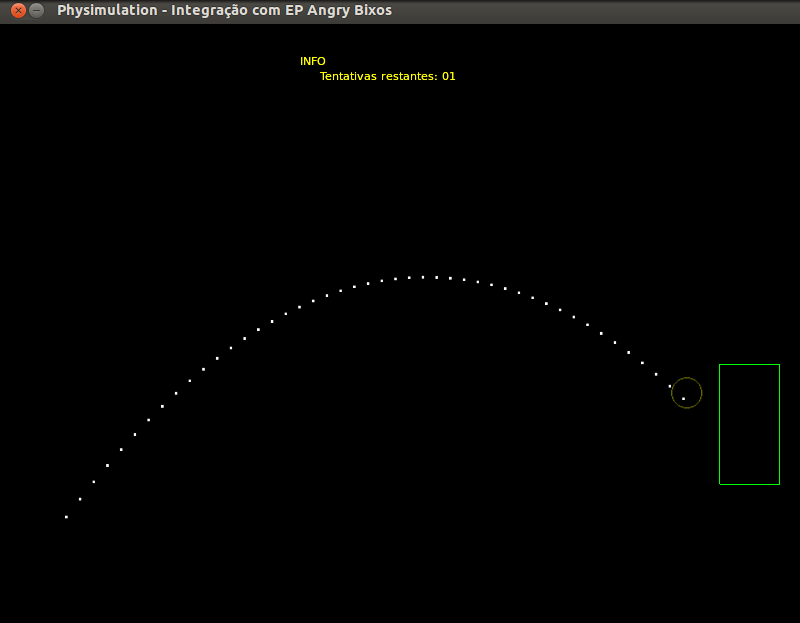
\includegraphics[scale=0.22]{images/angry-bixos-4E.png}
	\caption{Integração com EP Angry Bixos}
\end{figure}

\subsection{Apolo}

\begin{itemize}
  \item z1) posição inicial de uma nave em coordenadas cartesianas;                    
  \item z2) as componentes (V\_X,V\_Y) do vetor velocidade inicial da nave;
  \item z3) tempo máximo de simulação;               
  \item z4) o intervalo dT entre um instante e o instante seguinte da simulação.
\end{itemize}

\begin{figure}[H]
    \centering
	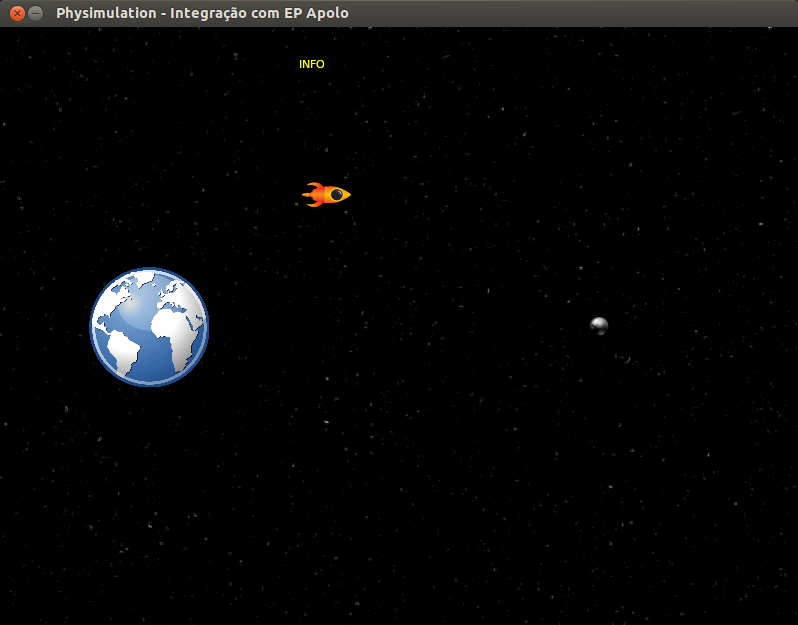
\includegraphics[scale=0.22]{images/apolo-4.png}
	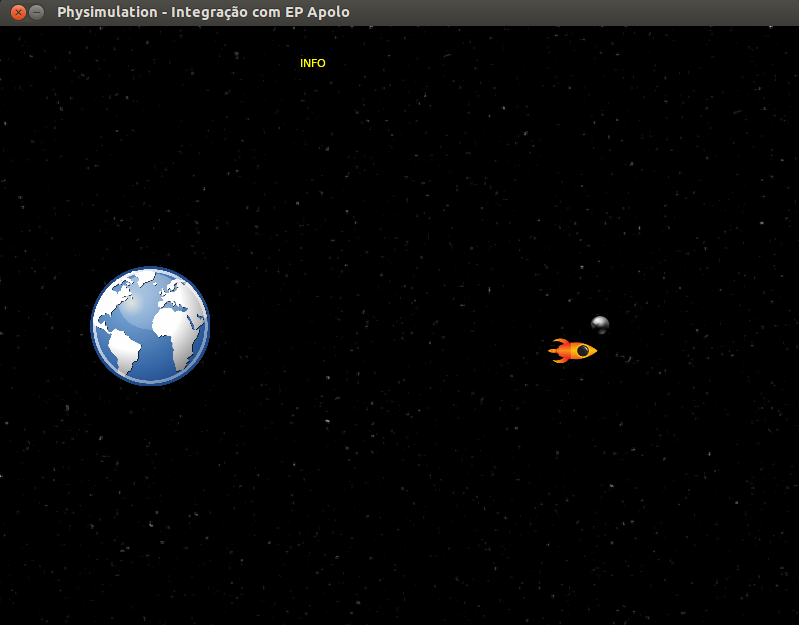
\includegraphics[scale=0.22]{images/apolo-6.png}
	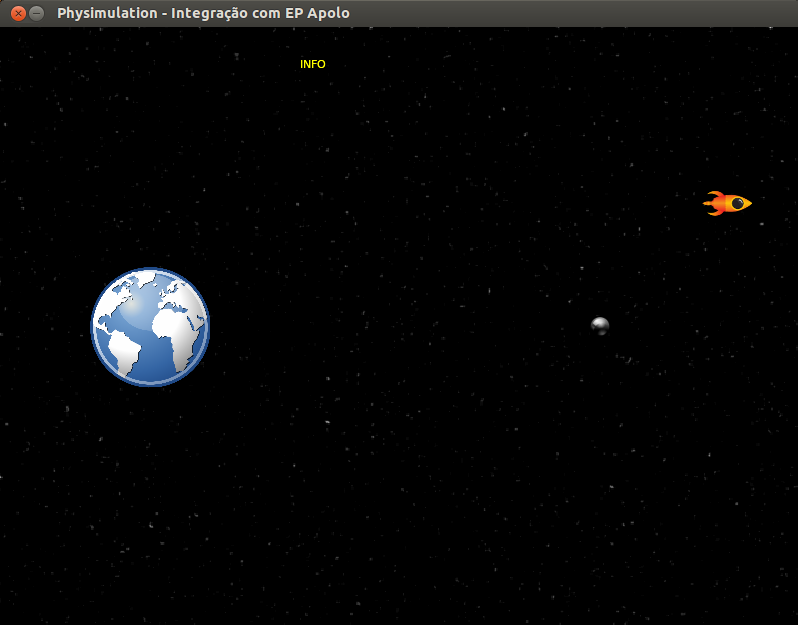
\includegraphics[scale=0.22]{images/apolo-3.png}
	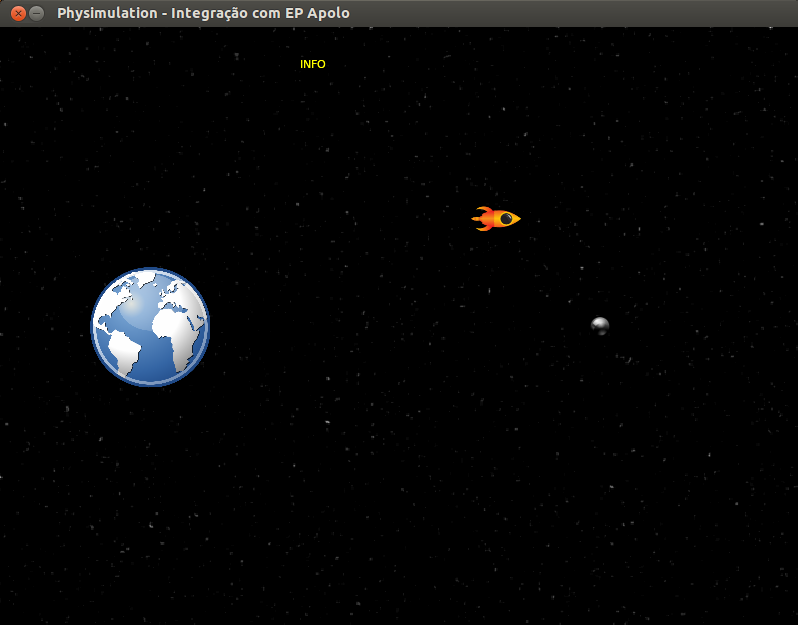
\includegraphics[scale=0.22]{images/apolo-2.png}
	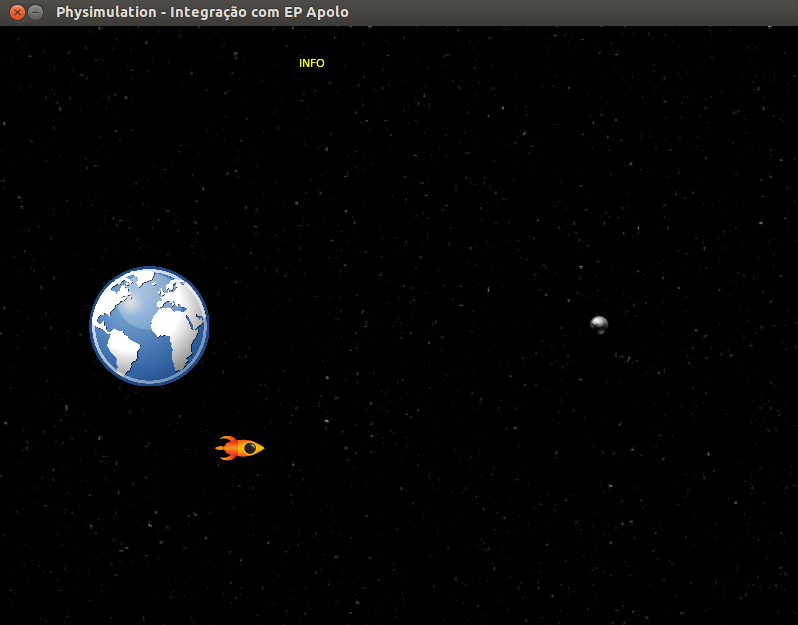
\includegraphics[scale=0.22]{images/apolo-1.png}
	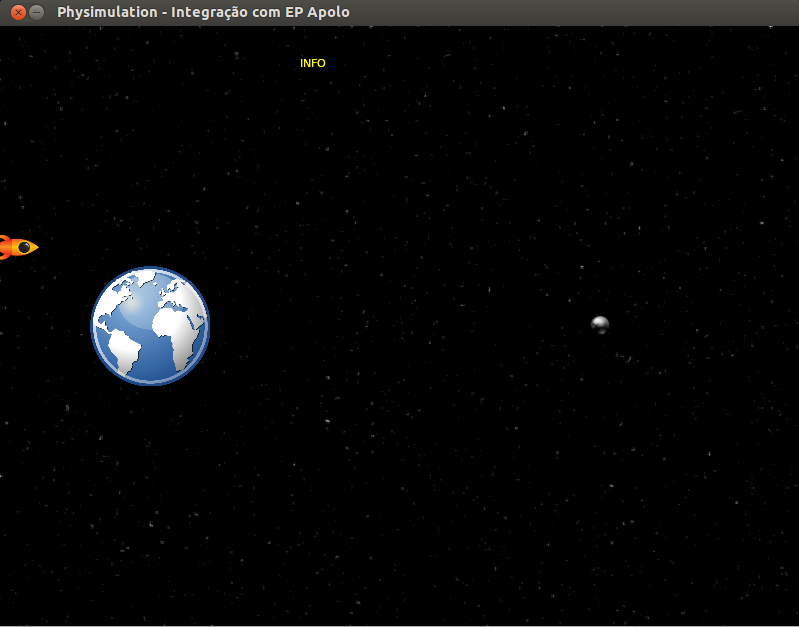
\includegraphics[scale=0.22]{images/apolo-5.png}
	\caption{Efeito \textit{slingshot} Integração com EP Apolo}
\end{figure}


